\documentclass{article}
\usepackage[utf8]{inputenc}
\usepackage[english]{babel}
\usepackage{amsmath}
\usepackage{graphicx}
\usepackage{float}
\usepackage{subfig}
 
\usepackage{multicol}
 
\begin{document}
\title{Formelark FYS2160}
\begin{multicols}{2}
\section*{Lover}
\begin{enumerate}
\setcounter{enumi}{-1}
\item $A\sim B$ og $B\sim C$ gir $A\sim C$
\item $\Delta E=Q+W$
\item $\Delta S\ge 0 \qquad$ Isolert system
\item $\lim_{\text{T} \to 0}\Rightarrow S = \text{konstant}$
\end{enumerate}

\section*{Mye brukte formler}
$$\begin{aligned}
F&=&E-TS\qquad&\text{Helmholtz}\\
G&=&E-TS+PV\qquad&\text{Gibbs}\\
\end{aligned}$$

$$\begin{aligned}
&F=-kT\ln(Z)\\
&\bigg(P+\frac{aN^2}{V^2}\bigg)(V-Nb)=NkT\\
&\ln N! \approx N\ln N - N\\
&S\equiv k\ln\Omega\\
&\Delta S_{\text{mixing}}=k\ln\binom{N}{N_A}\\
&W_{AB}=W_B-W_A=\int_{V_A}^{V_B}P(V)DV\\
&E=-kT^2\bigg(\frac{\partial\ln Z}{\partial T}\bigg)\\
\end{aligned}$$

\subsection*{Ideell gass}
$$\begin{aligned}
&PV=NkT\\
&\Delta S=\frac{dE}{T}=\frac{Q}{T}=\frac{C_VdT}{T}\\
&S=Nk\Bigg[\ln\Bigg(\frac{V}{N}\bigg(\frac{4\pi mE}{3Nh^2}\bigg)^{3/2}\Bigg)+\frac{5}{2}\Bigg]\\
\end{aligned}$$
\columnbreak
\subsection*{Multiplisitet}
$$\begin{aligned}
&\Omega(N_{\uparrow})=\binom{N}{N_{\uparrow}}=\frac{N!}{N_{\uparrow}!N_{\downarrow}}\qquad&\text{Paramagnet}\\
&\Omega(N,q)=\binom{q+N-1}{q}=\frac{(q+N-1)!}{q!(N-1)!}\qquad&\text{Einsteinkrystall}\\
&\Omega_N=\frac{1}{N!}\frac{V^N}{h^{3N}}\frac{2\pi^{3N/2}}{(3N/2-1)!}(\sqrt{2mE})^{3N-1}\qquad&\text{Ideell gass}
\end{aligned}$$
\subsection*{Varmeutveksling}
$$\begin{aligned}
&e&\equiv&\frac{W}{Q_h}=1-\frac{Q_c}{Q_h}\qquad&\text{Effektivitet varmemaskin}\\
&e&\equiv&\frac{Q_c}{W}=\frac{1}{Q_h/Q_c-1}\qquad&\text{Effektivitet kj{\o}lemaskin}\\
&\frac{dP}{dT}&=&\frac{S_g-S_l}{V_g-V_l}=\frac{L}{T\Delta V}\qquad&\text{Clausius-Clapeyron}\\
\end{aligned}$$
\subsection*{Kanonisk}
$$\begin{aligned}
&P&=&\frac{1}{Z}\exp(-\epsilon_i/kT)\qquad&\text{Boltzmannsfordelingen}\\
&Z&=&\sum_i\exp(-\epsilon_i/kT)\qquad&\text{Partisjonsfunksjonen}\\
&Z_N&=&\frac{Z_1^N}{N!}\qquad&\text{Total partisjon}\\
\end{aligned}$$
\subsection*{Grand-kanonisk}
$$\begin{aligned}
&\mathcal{Z}=\sum_N\sum_i \exp-[\epsilon_i-N\mu]/kT\qquad&\text{Gibbs sum}\\
&\bar{n}_{FD}=\frac{1}{\exp[(\epsilon-\mu)/kT]+1}\qquad&\text{Fermi-Dirac}\\
&\bar{n}_{BE}=\frac{1}{\exp[(\epsilon-\mu)/kT]-1}\qquad&\text{Bose-Einstein}\\
&\bar{n}_{B}=\exp[-(\epsilon-\mu)/kT]\qquad&\text{Boltzmann}\\
&E=\int_0^{\infty}\epsilon\bar{n}(\epsilon,\mu,T)D(\epsilon)d\epsilon\\
&N=\int_0^{\infty}\bar{n}(\epsilon,\mu,T)D(\epsilon)d\epsilon
\end{aligned}$$


\section*{Begreper}
\subsection*{Isokor}
Romlige dimensjoner (Volum, areal, lengde) holdes konstant
\subsection*{Isoterm}
Temperaturen holdes konstant
\subsection*{Isobar}
Trykket holdes konstant
\subsection*{Kvasistatisk}
En prosess som skjer så sakte at systemet blir værende i likevekt.
\subsection*{Adiabatisk}
Ingen endring i varme, i de fleste tilfeller heller ingen endring i entropi.
\subsection*{Isentropisk}
Adiabatisk og kvasistatisk
\subsection*{Likevekt}
\begin{itemize}
\item Mekanisk likevekt - $dP=0$
\item Termisk likevekt - $dT=0$
\item Diffusiv likevekt - $d\mu=0$
\item Kjemisk likevekt - $dG=0$
\end{itemize}
\columnbreak
\subsection*{Maxwellrelasjoner}
Relasjoner bygget på Schwarz' teorem:
\begin{equation*}
{\frac {\partial }{\partial x}}\left({\frac {\partial f}{\partial y}}\right)={\frac {\partial }{\partial y}}\left({\frac {\partial f}{\partial x}}\right)
\end{equation*}

\subsubsection*{Eksempler:}
$$\begin{aligned}+\left({\frac  {\partial T}{\partial V}}\right)_{S}&=&-\left({\frac  {\partial P}{\partial S}}\right)_{V}\\
+\left({\frac  {\partial T}{\partial P}}\right)_{S}&=&+\left({\frac  {\partial V}{\partial S}}\right)_{P}\\
+\left({\frac  {\partial S}{\partial V}}\right)_{T}&=&+\left({\frac  {\partial P}{\partial T}}\right)_{V}\\
-\left({\frac  {\partial S}{\partial P}}\right)_{T}&=&+\left({\frac  {\partial V}{\partial T}}\right)_{P}\end{aligned}$$

\subsection*{Nyttige sammenhenger:}
\begin{itemize}
\item Konstant energi og volum \newline
$\Rightarrow\Delta S>0$
\item Konstant temperatur og volum \newline
$\Rightarrow\Delta F<0$
\item Konstant temperatur og trykk \newline
$\Rightarrow\Delta G<0$
\end{itemize}

\section*{Differensialer}
$$\begin{aligned}
\frac{1}{T}&\equiv&\bigg(\frac{\partial S}{\partial E}\bigg)_{N,V}\\
C_V&\equiv&\bigg(\frac{\partial E}{\partial T}\bigg)_{N,V}\\
P&=&+T\bigg(\frac{\partial S}{\partial V}\bigg)_{E,N}&=&-\bigg(\frac{\partial F}{\partial V}\bigg)_{T,N}\\
\mu&=&-T\bigg(\frac{\partial S}{\partial N}\bigg)_{E,V}&=&+\bigg(\frac{\partial F}{\partial N}\bigg)_{T,V}&=&\bigg(\frac{\partial G}{\partial N}\bigg)_{T,P}\\
S&=&-\bigg(\frac{\partial F}{\partial V}\bigg)_{T,N}&=&-\bigg(\frac{\partial F}{\partial T}\bigg)_{V,N}&=&-\bigg(\frac{\partial G}{\partial T}\bigg)_{P,N}\\
V&=&\bigg(\frac{\partial G}{\partial P}\bigg)_{T,N}
\end{aligned}$$

\section*{Identiteter}
$$\begin{aligned}
dE&=&TdS-PdV+\mu dN\\
dF&=&-SdT-PdV+\mu dN\\
dG&=&-SdT+VdP+\mu dN
\end{aligned}$$

\section*{Utledninger}
\subsection*{Den termodynamiske identitet}
\begin{enumerate}
\item Tar utgangspunkt i $dQ=TdS$
\item T1L: $dE=dQ+dW$
\item $dW=PdV=\sigma dA=KdX$
\item Kan legge til $\mu dN$
\end{enumerate}
$\Rightarrow TdS=dE-PdV+\mu dN$

\subsection*{Energi rett fra Z}
Utgangspunkt:
$$Z(N,V,T)=\sum_i^N \exp(-\epsilon_i/kT)$$
$$P=(1/Z)\exp(-\epsilon_i/kT)$$

$$E=\sum_i^N\epsilon_i P(\epsilon_i)=(1/Z)\sum_i^N\epsilon_i\exp(-\epsilon_i\beta)$$
$$=\frac{1}{Z}\sum_i^N-\frac{\partial}{\partial\beta}\exp(-\epsilon_i\beta)=-\frac{1}{Z}\frac{\partial Z}{\partial\beta}$$
$$=-\frac{d\ln Z}{d\beta}=kT^2\bigg(\frac{\partial\ln Z}{\partial T}\bigg)$$

\subsection*{Adiabat for ideell gass}
\begin{enumerate}
\item Ta utgangspunkt i Sackur-Tetrode
\item Adiabat - $dS=0 \Rightarrow S_1=S_2$
\item Bruk ekvipartisjonsprinsippet
\end{enumerate}
$$\Rightarrow V_1^{2/3}T_1=V_2^{2/3}T_2$$

\subsection*{Clausius-Clapeyron}
\begin{enumerate}
\item $G_l=G_g$
\item $G_l(P_0+dP,T_0+dT)=G_g(P_0+dP,T_0+dT)$
\item Taylor: 
$$G_l(P_0+dP,T_0+dT)\approx G_l(P_0,T_0)$$
$$+\bigg(\frac{\partial G_l}{\partial P}\bigg)dP+\bigg(\frac{\partial G_l}{\partial T}\bigg)dT$$
\item Bruker differensialene
$$\bigg(\frac{\partial G_l}{\partial P}\bigg)_T=V_l,\quad\bigg(\frac{\partial G_l}{\partial T}\bigg)_P=-S_l$$
\end{enumerate}
$$\Rightarrow V_ldP-S_ldT=V_gdP-S_gdT$$
$$\Rightarrow \frac{dP}{dT}=\frac{S_l-S_g}{V_l-V_g}=\frac{L(T)}{T\Delta V}$$

\subsection*{Bose-Einstein-fordelingen}
\begin{enumerate}
\item Tar utgangspunkt i $$\mathcal{Z}=\sum_i^N\exp[-(n\epsilon-n\mu)/kT]$$
\item Bruker at $n=1,2,3...$
\item Bruker $\sum_nq^n=1/(1-q),\, q<1$
\item $\bar{n}=\sum nP(n)$
\end{enumerate}
$$\Rightarrow \frac{1}{\mathcal{Z}}\sum_n n\exp(-nx)=\frac{1}{\mathcal{Z}}\sum_n\frac{\partial}{\partial x}\exp(-nx)$$
$$\Rightarrow \frac{1}{\mathcal{Z}}\frac{\partial\mathcal{Z}}{\partial x}=\frac{1}{\exp[(\epsilon-\mu)/kT]-1}$$
\end{multicols}

\begin{figure}%
    \centering
    \subfloat[Carnotsyklusen]{{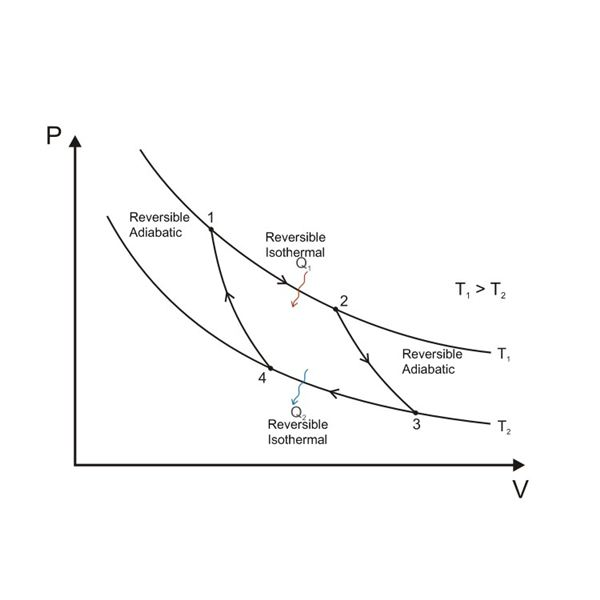
\includegraphics[width=6cm]{carnot.jpg} }}%
    \qquad
    \subfloat[Faseoverganger for rene substanser]{{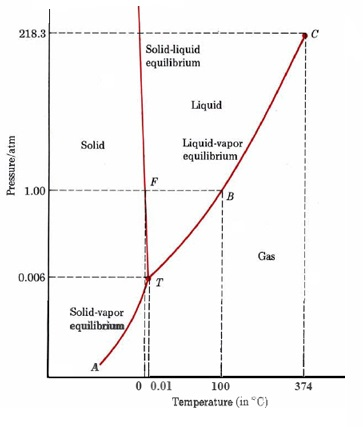
\includegraphics[width=5cm]{triple.jpg} }}%
\end{figure}

\begin{figure}[h]
\centering
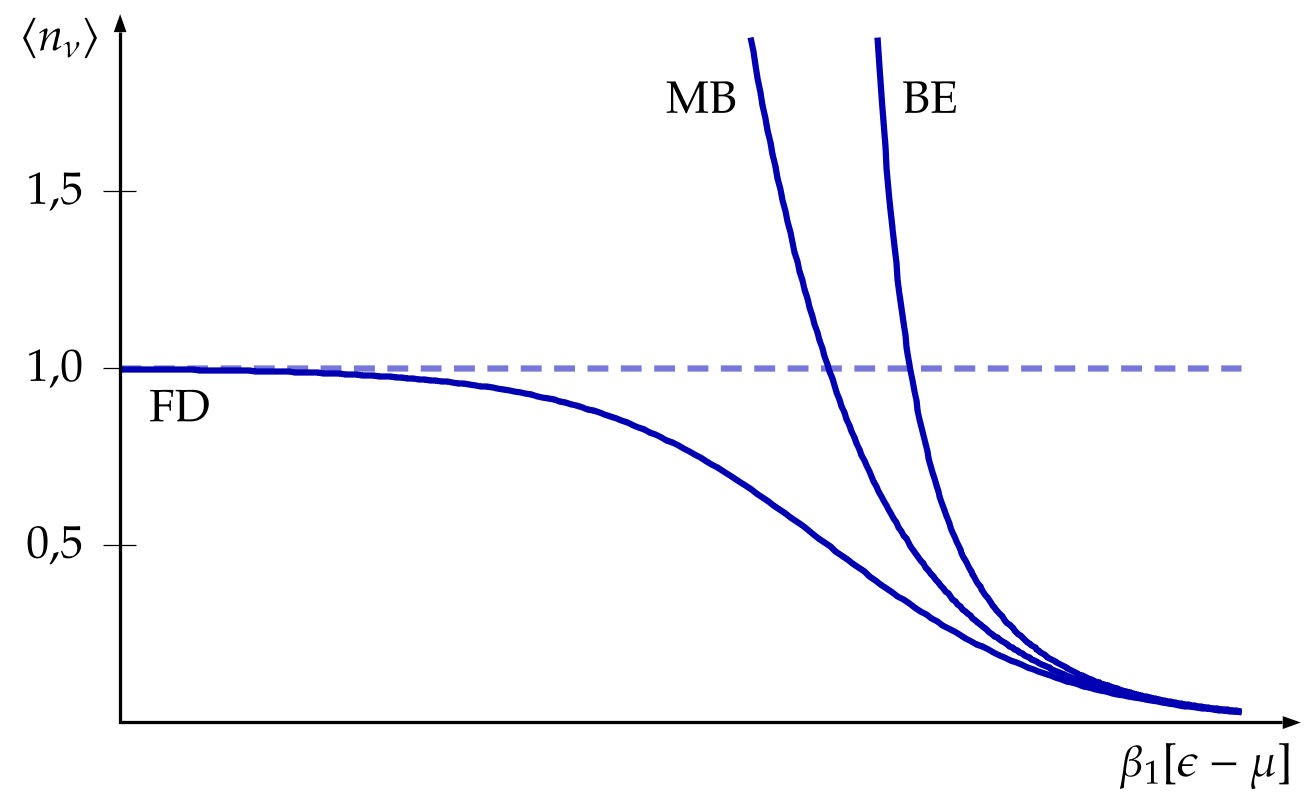
\includegraphics[width=90mm]{fordelinger.png}
\caption{Fordelingsfunksjoner (Fermi-Dirac, Boltzmann, Bose-Einstein)}
\end{figure}
\subsection*{Tilstandstettheten og fermienergi}
\subsubsection*{3D:}
$$D(n)dn=N_T\cdot A=2\cdot (1/8)\cdot 4\pi n^2dn=\pi n^2dn\qquad N_T=2\text{ for fermioner}$$
$$\Rightarrow D(n)dn=D(\epsilon)d\epsilon\Rightarrow D(\epsilon)=\pi n^2(1/2an)=\frac{\pi}{2a}n=\frac{\pi}{2a}\sqrt{\frac{\epsilon}{a}}$$
$$N=N_T\cdot V(n_{max})=2\cdot\frac{1}{8}\cdot\frac{4}{3}\pi n_{max}^3\quad\Rightarrow n_{max}^2=\bigg(\frac{3N}{\pi}\bigg)^{2/3}$$
$$\epsilon_F=\epsilon(n_{max})=an_{max}^2=a\bigg(\frac{3N}{\pi}\bigg)^{2/3}$$ 
\end{document}